% !TEX root = main.tex

\section{语法分析}
\subsection{上下文无关法}
语法分析需要解决:从词法分析中获得的每个属性字(token)在语句中承担什么角色,同时检查语句是否符合程序语言的语法。

很多语言并非是正则的,比如匹配的括号串$\{(^i)^i\mid i\geq 0\}$,原因是FA不能记住其访问某一状态的次数,因此需要有更加强大的语言。

\begin{definition}[上下文无关法(context-free gramma, CFG)]
包括四部分
\begin{itemize}
	\item 终端符号(terminal)的集合$T$
	\item 非终端符号的集合$N$
	\item 唯一的开始符号$S\in N$
	\item 若干以下形式的产生式(production)
	\[X\to Y_1Y_2\ldots Y_n\]
	其中$X\in N$且$Y_i\in T\cup N\cup\{\epsilon\}$。
	多个左侧相同的产生式右侧可用$\mid$合并。
\end{itemize}
\end{definition}
\begin{definition}[推导(derivation)]
从开始符号开始,每一步推导就是用一个产生式的右方取代左端的非终端符号。
\end{definition}

CFG定义语言的能力比正则表达式强很大原因是它引入了\textbf{递归}的因素。

\begin{example}
用上下文无关文法定义下列语言:
\begin{itemize}
	\item $L=\{0^n1^n\mid n\geq 1\}$:$E\to 0E1\mid 01$
	\item 只含有$0$和$1$的回文串:$S\to 0S0\mid 1S1\mid 0\mid 1\mid \epsilon$
	\item 只含有$($和$)$的匹配括号串:$E\to (E)\mid EE\mid \epsilon$
\end{itemize}
\end{example}

\begin{itemize}
	\item 最左推导:每步推导都替换最左侧的非终端符号
	\[E\xRightarrow{lm}
	-E\xRightarrow{lm}
	-(E)\xRightarrow{lm}
	-(E+E)\xRightarrow{lm}
	-(id+E)\xRightarrow{lm}
	-(id+id)\]
	\item 最右推导:每步推导都替换最右侧的非终端符号
	\[E\implies
	-E\implies
	-(E)\implies
	-(E+E)\implies
	-(E+id)\implies
	-(id+id)\]
\end{itemize}

\begin{definition}[二义性]
如果对于一个文法,存在一个句子,对这个句子可以构造两棵不同的分析树,那么我们称这个文法为二义的。
\end{definition}
看语法分析树的叶子结点能不能连成句子。

\begin{example}
对于文法$E\to E+E\mid E*E\mid -E\mid (E)\mid id$及句子$id+id*id$,有以下两种推导:

\begin{minipage}{0.5\linewidth}
\[\begin{aligned}
E &\implies E+E\\
&\implies id+E\\
&\implies id+E*E\\
&\implies id+id*E\\
&\implies id+id*id\\
\end{aligned}\]
\end{minipage}
\begin{minipage}{0.5\linewidth}
\[\begin{aligned}
E &\implies E+E\\
&\implies id+E\\
&\implies id+E*E\\
&\implies id+id*E\\
&\implies id+id*id\\
\end{aligned}\]
\end{minipage}
\end{example}

文法二义性的消除可通过引入更多的产生式。
\begin{example}
$E\to E+E\mid E*E\mid (E)\mid id$是有二义的,因为不知道应该先算加法还是乘法。
可将其改为
\[\begin{aligned}
E &\to E+T\mid T\\
T &\to T*F\mid F\\
F &\to (E)\mid id
\end{aligned}\]
其中$E$为Expression,$T$为Term,$F$为Facotr,即可消除二义性(必然得先算乘法)。
相当于先算$F$,再算$T$,最后算$E$。
\end{example}
\begin{example}
悬挂的if-else:\verb'if E1 then if E2 then E3 else E4',可以令\verb'else'匹配最近的\verb'then'。
\[\begin{array}{rll}
E &\to MIF &\text{//所有的then都被匹配}\\
  &\mid UIF &\text{//仅有一些then}\\
MIF &\to \text{if } E \text{ then } MIF \text{ else } MIF &\\
  &\mid OTHER &\\
UIF &\to \text{if } E \text{ then } E &\\
  &\mid \text{if } E \text{ then } MIF \text{ else } UIF &
\end{array}\]
\end{example}

并不是所有上下文无关文法都可以做到无二义,也无法判断一个上下文无关文法是否是二义的。

\subsection{NFA转CFG}
\begin{enumerate}
	\item 对于NFA的每一状态$i$,创建非终态$A_i$
	\item 若状态$i$在输入$a$上有转换边到状态$j$,则添加生成式$A_i\to aA_j$;
	若状态$i$在输入$\epsilon$上转换到状态$j$,则添加生成时$A_i\to A_j$
	\item 若$i$是接受状态,则添加$A_i\to\epsilon$
	\item 若$i$是初始状态,则令$A_i$为语法的初始符号
\end{enumerate}

\begin{definition}[右线性文法]
如果每个产生式都属于下列形式之一
\[A\to aB\qquad A\to a\qquad A\to\epsilon\]
则这样的文法称为右线性文法
\end{definition}
\begin{definition}[左线性文法]
如果每个产生式都属于下列形式之一
\[A\to Ba\qquad A\to a\qquad A\to\epsilon\]
则这样的文法称为左线性文法
\end{definition}

在处理程序时,上下文无法文法存在局限性,无法解决诸如以下问题:
\begin{itemize}
\item 变量先声明,再使用
\item 调用函数时,实参个数和形参个数一致
\end{itemize}
都得留到语义分析阶段才解决。

\subsection{递归下降}
递归下降语法翻译即从顶层的非终端符号$E$开始,顺序尝试$E$的所有规则,完整例子可见\href{http://web.stanford.edu/class/cs143/lectures/lecture06.pdf}{此文档},但需要先消除左递归。

\begin{definition}[左递归]
对于非终端符号$A$有生成式$A\to A\alpha$,则该文法是左递归的。
\end{definition}
消除左递归的方法:
\[A\to A\alpha_1\mid \cdots\mid A\alpha_m\mid\beta_1\mid\cdots\beta_n
\implies
\begin{aligned}
A &\to\beta_1 A'\mid\cdots\mid\beta_n A'\\
A' &\to\alpha_1 A'\mid\cdots\mid\alpha_m A'\epsilon
\end{aligned}\]

\begin{definition}[FIRST集与FOLLOW集]
$FIRST(\alpha)$集为从$\alpha$中推导出来的字符串第一个终端符号的集合,若$\alpha\to\epsilon$,则$\epsilon\in FIRST(\alpha)$;若$A\to c\gamma$,则$c\in FIRST(A)$。
$FOLLOW(A)$集为可以出现在$A$右侧的终端符号的集合。
若$A$是最右端的符号,则字符串结束符号$\$\in FOLLOW(A)$。
\end{definition}

\begin{myalgorithm}
计算$FIRST(X)$集
\begin{enumerate}
	\item 如果$X$是终端符号,则$FIRST(X)=\{X\}$
	\item 如果$X$是非终端符号,且$X\to Y_1Y_2\cdots Y_k$。
\begin{itemize}
	\item 若$Y_1\cdots Y_{i-1}\to\epsilon$,则将$a\in FIRST(Y_i)$放入$FIRST(X)$。
	\item 若$\epsilon\in FIRST(Y_j),j=1,2,\ldots,k$,则将$\epsilon$放入$FIRST(X)$中。
\end{itemize}
	\item 若$X\to\epsilon$是生成式,将$\epsilon$放入$FIRST(X)$中
\end{enumerate}
\end{myalgorithm}

\begin{myalgorithm}
计算$FOLLOW(A)$集
\begin{enumerate}
	\item 将$\$$放入$FOLLOW(S)$,其中$S$是开始符号
	\item 如果有生成式$A\to\alpha B\beta$,那么$\forall a\in FIRST(\beta),a \ne\epsilon:\;a\in FOLLOW(B)$
	\item 如果有生成式$A\to\alpha B$,或生成式$A\to\alpha B\beta$,且$\epsilon\in FIRST(\beta)$,则$\forall a\in FOLLOW(A):\;a\in FOLLOW(B)$
\end{enumerate}
\end{myalgorithm}

简而言之,$FOLLOW$集看下一符号的$FIRST$,如果$\epsilon$在下一符号的$FIRST$集中,则看生成式左端的$FOLLOW$集。

另一种方式:
\begin{enumerate}
	\item \$$\in FOLLOW(S)$
	\item $\forall A\to\alpha X\beta:\;FIRST(\beta)-\{\epsilon\}\subset FOLLOW(X)$
	\item $\forall A\to\alpha X\beta,\epsilon\in FIRST(\beta):\;FOLLOW(A)\subset FOLLOW(X)$
\end{enumerate}

\begin{figure}[H]
\centering
\begin{tabular}{c}
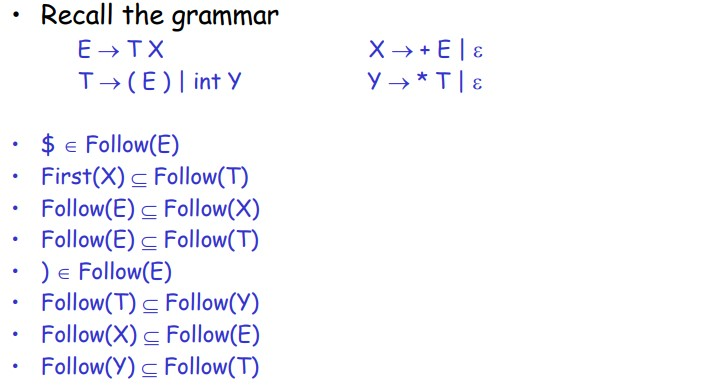
\includegraphics[width=0.8\linewidth]{fig/follow_eg1.jpg}\\
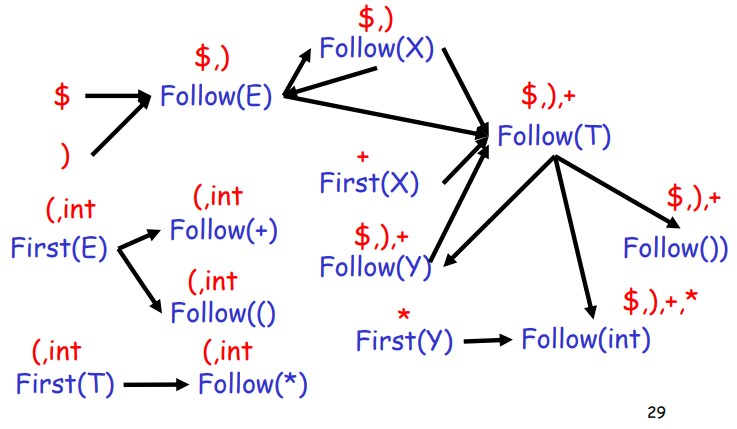
\includegraphics[width=0.8\linewidth]{fig/follow_eg2.jpg}
\end{tabular}
\end{figure}

\subsection{预测分析}
LL(1)文法
\begin{itemize}
	\item 第一个L:输入字符串从左边开始扫描
	\item 第二个L:得到的推导是最左推导
	\item (1):向前看1个输入符号(或单词)
\end{itemize}

递归下降在每一步都会有多种生成式的选择,这会导致大量的回溯。
而在LL(1)文法中,每一步都只有一种生成式的选择,避免了回溯。

左因子分解(left-factoring)将生成式的\textbf{共同前缀}分解出来。
\begin{example}
考虑以下文法
\[\begin{aligned}
E &\to T + E\mid T\\
T &\to int \mid int * T\mid (E)
\end{aligned}\]
共同前缀分解后即得
\[\begin{aligned}
E &\to TX\\
X &\to +E\mid \epsilon\\
T &\to int\;Y\mid (E)\\
Y &\to *T\mid \epsilon
\end{aligned}\]
有LL(1)语法表,其中最左列为最左非终端符号,最上行为下一输入符号,表格内容为使用的右端生成式。
\begin{center}
\begin{tabular}{|c|c|c|c|c|c|c|}\hline
 & $int$ & $*$ & $+$ & $($ & $)$ & \$\\\hline
$E$ & $TX$ & & & $TX$ & & \\\hline
$X$ &  &  & $+E$ & & $\epsilon$ & $\epsilon$\\\hline
$T$ & $int\; Y$ & & & $(E)$ & &\\\hline
$Y$ &  & $*T$ & $\epsilon$ & & $\epsilon$ & $\epsilon$\\\hline
\end{tabular}
\end{center}
\end{example}

基于表的预测语法分析,用栈实现。
\begin{algorithm}
\caption{Table-Driven Predictive Parsing}
\begin{algorithmic}[1]
\State \verb'ip=0'
\State \verb'X=stack.top()'
\While {$X\ne\$$}
\If {X == w[ip]}
\State \verb'stack.pop(); ip++;'
\Else \If {X is a terminal or M[X,a]=$\varnothing$}
\State Error()
\Else
\State Output production \verb'M[X,a]'$=X\to Y_1Y_2\cdots Y_k$
\State stack.pop()
\State push $Y_k,Y_{k-1},\ldots,Y_1$ onto the stack
\EndIf
\EndIf
\State \verb'X=stack.top()'
\EndWhile
\If {w[ip] != '\$'}
\State Error()
\EndIf
\end{algorithmic}
\end{algorithm}

\subsection{移进-规约}
自底向上的语法分析采用两种动作:
\begin{itemize}
\item 移进(shift):将\verb'|'向右移动一格
\[ABC\mid xyz\implies ABCx\mid yz\]
\item 规约(reduce):在字符串右侧逆向应用生成式
\[Cbxy\mid ijk\implies CbA\mid ijk\]
\end{itemize}

\begin{figure}[H]
\centering
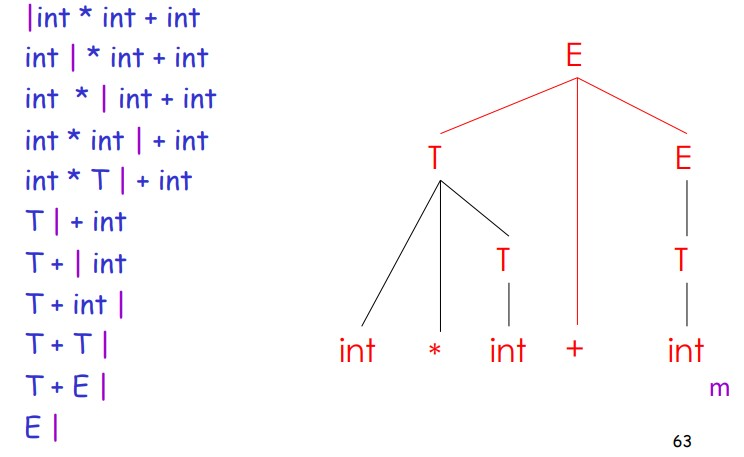
\includegraphics[width=0.8\linewidth]{fig/shift-reduce.jpg}
\end{figure}
移进将终端符号移入栈中,规约将生成式的右端符号弹出,将生成式的左端\textbf{非终端}符号推入。

\begin{definition}[句柄(handle)]
A handle is a string that can be reduced and also allows further reductions back to the start symbol.
\end{definition}

\begin{definition}[活前缀(viable prefix)]
$\alpha$是活前缀若存在$\omega$使得$\alpha\mid\omega$是移进-规约语法分析器的状态。
\end{definition}

LR(0)语法:
\begin{itemize}
	\item 栈包含$\alpha$,下一输入是$t$,DFA在输入$\alpha$上终止在状态$s$
	\item 当$s$包含$X\to\beta$的项时进行规约
	\item 当$s$包含$X\to\beta.t\omega$的项时移进
\end{itemize}

LR(0)可能存在以下两种冲突:
\begin{itemize}
	\item 规约-规约冲突:$X\to\beta.$且$Y\to\omega.$
	\item 移进-规约冲突:$X\to\beta.$且$Y\to\omega.t\delta$
\end{itemize}

\begin{example}[用NFA识别活前缀]
考虑以下文法:
\[\begin{array}{rrll}
(1) & E &\to & E+T\\
(2) & E &\to & T\\
(3) & T &\to & TF\\
(4) & T &\to & F\\
(5) & F &\to & F^*\\
(6) & F &\to & a\\
(7) & F &\to & b
\end{array}\]
构造识别这一文法所有活前缀(viable prefixes)的LR(0)自动机.
\begin{figure}[H]
\centering
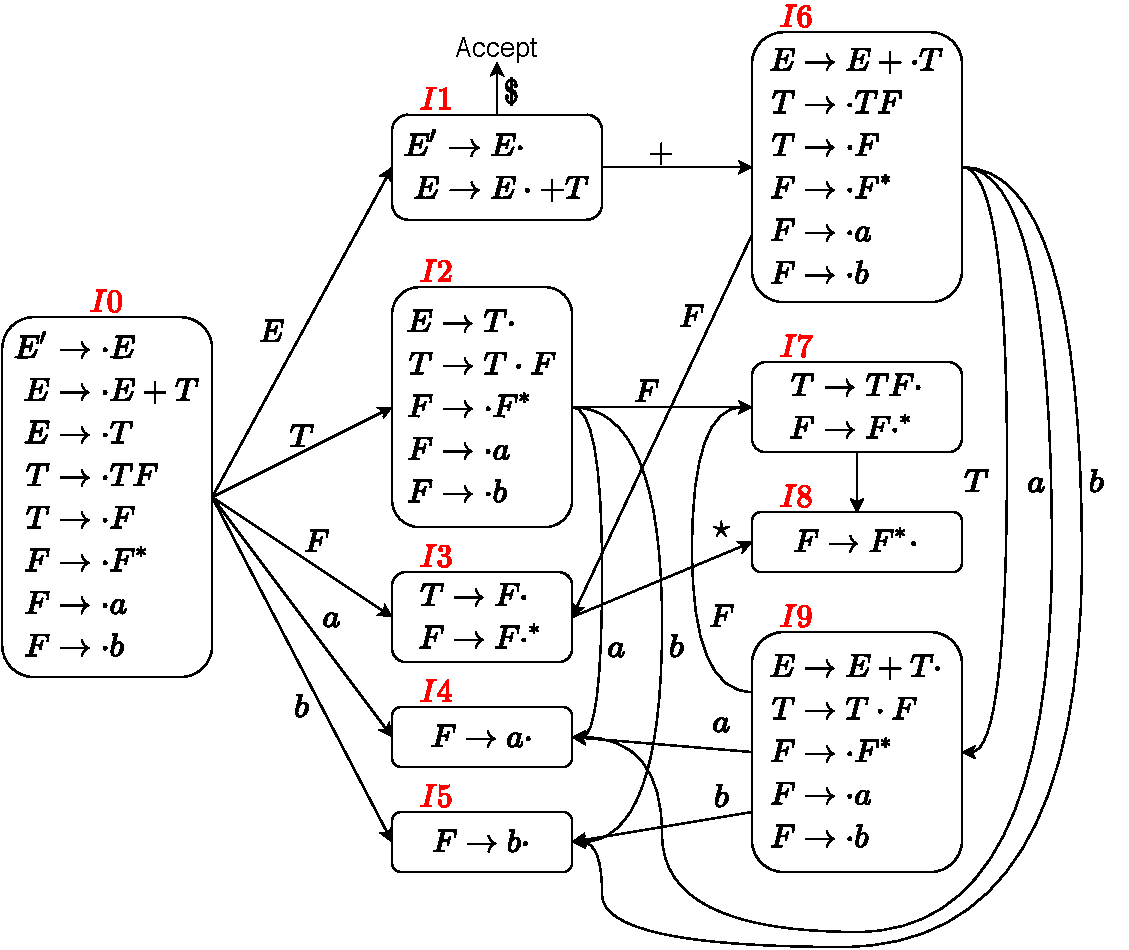
\includegraphics[width=0.8\linewidth]{fig/T06.pdf}
\end{figure}
\end{example}

SLR(simple left-to-right scan)用启发式算法提升了LR(0)移进规约的效率,减少冲突。
\begin{itemize}
	\item 栈包含$\alpha$,下一输入是$t$,DFA在输入$\alpha$上终止在状态$s$
	\item 当$s$包含$X\to\beta$的项且\textcolor{red}{$t\in FOLLOW(X)$}时进行规约
	\item 当$s$包含$X\to\beta.t\omega$的项时移进
\end{itemize}

\subsection{语法制导翻译}
抽象语法树(Abstract Syntax Trees, AST)是将原本语法树中冗余的成分给去除,比如左右括号原本都是各自一个结点,但在AST中不会呈现。

语法制导翻译(syntax-directed translation)给语法符号提供了属性(attribute),给生成式提供了动作(action)。
\begin{example}
对下列语法进行求值
\[E\to int\mid E+E\mid (E)\]
有语法制导定义
\begin{center}
\begin{tabular}{ll}
$E\to int$ & $E.val=int.val$\\
$E\to E_1+E_2$ & $E.val=E_1.val+E_2.val$\\
$E\to (E_1)$ & $E.val=E_1.val$
\end{tabular}
\end{center}
\end{example}

\begin{itemize}
\item 综合属性(synthesized):从后代计算得到
\item 继承属性(inherited):从语法树的父亲或兄弟中计算得到
\end{itemize}